\documentclass[10pt]{article}
%\documentclass[review]{siamart1116}
%\documentclass[review]{siamonline1116}

\usepackage{amsmath}
\usepackage{amsfonts}
\usepackage{amssymb}
\usepackage{fancyhdr}
\usepackage[margin=0.75in]{geometry}
\usepackage{graphicx}
\usepackage[section]{placeins}
\usepackage{nicefrac}
\usepackage{bm}
\usepackage{xcolor}
\usepackage[format=plain,indention=.5cm, font={it,small},labelfont=bf]{caption}
\usepackage{subcaption}
\usepackage{float}
\usepackage{enumerate}
\usepackage{tikz}
\usetikzlibrary{arrows.meta}
\usepackage[all]{xy}
\usepackage{url}



%%%%%%%%%%%%%%%%%%%%%%%%%%%%%%%%%%%%%%%%%%%%%%%%%%%%%%%%%%%%%%%%%%%%%%%%%%%%%%%%%%%%%%%%%%%%%%%%%%%%%%%%%%%%%%%%%%
\usepackage{stackengine}
\usepackage{amsthm}
\usepackage{cleveref}


\newtheorem{theorem}{Theorem}
\newtheorem*{theorem*}{Theorem}
\newtheorem{lemma}{Lemma}
\newtheorem*{lemma*}{Lemma}
\newtheorem{conj}{Conjecture}
\newtheorem{corollary}{Corollary}
\newtheorem{clm}{Claim}
\newtheorem{rmk}{Remark}
\newtheorem{note}{NOTE}
\newtheorem{method}{Method}

\theoremstyle{definition}
\newtheorem*{def*}{Definition}
\newtheorem{definition}{Definition}
\numberwithin{theorem}{section}
\numberwithin{definition}{section}
\numberwithin{lemma}{section}
\numberwithin{corollary}{section}
\numberwithin{clm}{section}
\numberwithin{rmk}{section}

\newcommand{\low}[1]{$_{\text{#1}}$}
\newcommand\xput[2][0.5]{%
	\rule{#1\linewidth}{0pt}\makebox[0pt][c]{#2}\hfill}

\setlength{\headheight}{15pt}
\pagestyle{fancy}
\renewcommand{\headrulewidth}{0pt}
\fancyhead[L]{Brunner}
\fancyhead[C]{Co-Occurrance Network}
\fancyhead[R]{\today}
\lfoot{}
\cfoot{\thepage}
\rfoot{}

%%%%%%%%%%%%%%%%%%%%%%%%%%%%%%%%%%%%%%%%%%%%%%%%%%%%%%%%%%%%%%%%%%%%%%%%%%%%%%%%%%%%%%%%%%%%%%%%%%%%%%%%%%%%%%%%%%
%
%
%\newsiamthm{clm}{Claim}
%\newsiamremark{rmk}{Remark}
%\newsiamremark{note}{NOTE}
%\numberwithin{theorem}{section}
%
%
%%%%%%%%%%%%%%%%%%%%%%%%%%%%%%%%%%%%%%%%%%%%%%%%%%%%%%%%%%%%%%%%%%%%%%%%%%%%%%%%%%%%%%%%%%%%%%%%%%%%%%%%%%%%%%%%%%
\newenvironment{inbox}[1]
{\begin{center}
		\begin{tabular}{|p{0.9\textwidth}|}
			\hline
			{\bf #1}\\
		}
		{ 
			\\\\\hline
		\end{tabular} 
	\end{center}
}
\newenvironment{inbox2}
{\begin{center}
		\begin{tabular}{|p{0.9\textwidth}|}
			\hline \vspace{-0.5 cm}
		}
		{ 
			\\ \hline
		\end{tabular} 
	\end{center}
}

\newcommand{\nhalf}{\nicefrac{1}{2}}
\newcommand{\eps}{\epsilon_{machine}}
\newcommand{\ol}{\overline}
\renewcommand{\b}{\bm}

\definecolor{dgreen}{RGB}{49,128,23}
\definecolor{lgreen}{RGB}{77, 255, 166}
\definecolor{nicepink}{RGB}{255, 0, 102}
\definecolor{nicered}{RGB}{255, 80, 80}
\definecolor{lblue}{RGB}{102, 163, 255}
\definecolor{lgray}{RGB}{217, 217, 217}

\newcommand{\bE}{\mathbb{E}}
\newcommand{\bP}{\mathbb{P}}
\newcommand{\bR}{\mathbb{R}}
\newcommand{\bN}{\mathbb{N}}
\newcommand{\bZ}{\mathbb{Z}}
\newcommand{\bQ}{\mathbb{Q}}
\newcommand{\bC}{\mathbb{C}}
\newcommand{\cA}{\mathcal{A}}
\newcommand{\cB}{\mathcal{B}}
\newcommand{\cC}{\mathcal{C}}
\newcommand{\cD}{\mathcal{D}}
\newcommand{\cE}{\mathcal{E}}
\newcommand{\cF}{\mathcal{F}}
\newcommand{\cG}{\mathcal{G}}
\newcommand{\cH}{\mathcal{H}}
\newcommand{\cI}{\mathcal{I}}
\newcommand{\cJ}{\mathcal{J}}
\newcommand{\cK}{\mathcal{K}}
\newcommand{\cL}{\mathcal{L}}
\newcommand{\cM}{\mathcal{M}}
\newcommand{\cN}{\mathcal{N}}
\newcommand{\cO}{\mathcal{O}}
\newcommand{\cP}{\mathcal{P}}
\newcommand{\cQ}{\mathcal{Q}}
\newcommand{\cR}{\mathcal{R}}
\newcommand{\cS}{\mathcal{S}}
\newcommand{\cT}{\mathcal{T}}
\newcommand{\cU}{\mathcal{U}}
\newcommand{\cV}{\mathcal{V}}
\newcommand{\cW}{\mathcal{W}}
\newcommand{\cX}{\mathcal{X}}
\newcommand{\cY}{\mathcal{Y}}
\newcommand{\cZ}{\mathcal{Z}}

\newcommand{\inter}{\text{\normalfont int}}
\newcommand{\ka}{\kappa}
\newcommand{\fp}{\varrho}
\newcommand{\problem}[2]{ \ \\ {\bf #1} {\it #2} \ \\} 

\renewcommand{\arraystretch}{1.5}
\renewcommand{\thefootnote}{\fnsymbol{footnote}}	
\author{Jim Brunner}
\title{Using a co-occurrance network}

\begin{document}
\maketitle
\section{Network Building}
We are looking at creating ecological networks of a microbiome. Right now, I have built two networks, in the form of graphs $\cG_1 = (\cV_1, \cE_1)$ and $\cG_2 = (\cV_2,\cE_2)$. In both graphs, vertex are labeled by taxa name. I'm going to conflate the vertices and their label. The edge sets are defined by co-incidence and co-occurence, respectively. Given a set of samples with abundancs of organisms, we map the abundances to discrete levels, as proportions of the maximum abundance \emph{of that organism}. Precisely, let the samples be $s_i$ and raw abundance of organism $j$ in sample $i$ be $r_{ji}$. I map the abundances according to
\[
a(r_{ji})  = \left\{
\begin{array}{c c}
\lfloor\left(\frac{r_{ji}}{\max_{s_k}(r_{jk})}\right) n \rfloor + 1 &  \frac{r_{ji}}{\max_{s_k}(r_{jk})} \geq m \\
0 & \frac{r_{ji}}{\max_{s_k}(r_{jk})} < m
\end{array}
\right.
\]
where $m$ is some minimum. Then, I create weighted edges between vertices (where $0$ weight means no edge exists) where the weights of edges in $\cE_1$ are
\[
w^1_{jk} = \frac{\|\{i: a(r_{ji}) = a(r_{ki}) \neq 0\} \|}{S}
\]
where $S$ is the total number of samples. That is, we count the propotion of samples in which the two taxa appear at the same discritized level. 

The second network accounts for random coincidence of taxa in a sample, following \cite{coocc}. It begins with $\cG_1$, and compares to a null model $N$. The null model is defined in the following way.
\[
A_j= \sum_{s_i} \b{1}_{a(r_{ji}) \neq 0}
\] 
and 
\[
S_i^l  = \sum_{v_j} \b{1}_{a(r_{ji}) = l}
\]
Then, $N$ assumes that if
\[
X_{jil} \sim \mathit{binom}\left(A_j, \frac{S_i^l}{\sum_{il} S_i^l}\right)
\]
then $P(a_{ji}^N = l) = 1-P(X_{jil} = 0)$. This allows us to calculate the probability of co-incidence of taxa under the null model. Let $w_{jk}^N$ be
\[
w^N_{jk} = \|\{i: a_{ji}^N = a_{ki}^N \neq 0\} \|
\]
This is the similar to the co-incidence model but now randomized. Then,
\[
P(w_{jk}^N = K) =  \sum_{\{A \subset \cV_2:|A| = k\}} \prod_{l\in A} a_{jl}a_{kl}\prod_{l \not\in A} (1- a_{jl}a_{kl})
\]
Ideally, we would then define $\cE_2$ by the weights
\[
w_{jk}^2 = \left\{ \begin{array}{c c}
1 & P(w_{jk}^N \geq w_{jk}^1) \leq t\\
0 & P(w_{jk}^N < w_{jk}^1) > t
\end{array}\right.
\]
However, that probability is intractible to compute. Instead, we take 
\[
\widetilde{P}(w_{jk}^N = K) = \sum_{l=0}^i \binom{N_1}{l}\binom{N_2}{K-l} p_1^j p_2^{K-l} (1-p_1)^{N-l}(1-p_2)^{N-K+l}
\]
where
\[
p_1 = p_a - \left(\frac{N_2}{N_1}\frac{N(\mu-\sigma^2)- \mu^2}{N^2}\right)^{\nhalf}
\]
and 
\[
p_2 = p_a - \left(\frac{N_1}{N_2}\frac{N(\mu-\sigma^2)- \mu^2}{N^2}\right)^{\nhalf}
\]
Finally, $N_1$, $N_2$ are to ensure that $p_1,p_2 \in [0,1]$. It turns out we need:
\[
\frac{\mu N (1-p_a) - N\sigma^2}{N(1-p_a)- \sigma^2} \leq N_2 \leq \frac{\mu^2}{\mu- \sigma^2}
\]
with $\mu$ the mean of the real distrubution, $\sigma^2$ the variance, and $p_a = \frac{1}{S}\sum_{i} a_{ji}a_{ki}$. So, we take 
\[
w_{jk}^2 = \left\{ \begin{array}{c c}
1 & \widetilde{P}(w_{jk}^N \geq w_{jk}^1) \geq t\\
0 & \widetilde{P}(w_{jk}^N < w_{jk}^1) > t
\end{array}\right.
\]

\subsection{An alternative coincidence construction}
A faster way would be to first normalize abundance vectors, and just take 
\[
W = AA^T
\]
(with the diagonal reset to 0) to be the weighted adjacency matrix, where $A$ is the matrix of abundances. Then, each entry is the cosine of the angle between the abundance vectors. This also allows us to look at negatively aligned abundance vectors.

How then would we construct the cooccurrence network? Basically, what would our null model be? Well, we would still randomize the sample data. That is, we could take $X_{ij}$ be a random variable representing the abundance of taxa $i$ in sample $j$, and require that $\|X_{i}\| = 1$. Then, we can ask $P(\b{X}_i \cdot \b{X}_k > w_{ik})$. I just don't know what distribution to put on the $X_{ij}$ (the random abundances). I'll start with a binomial:
\[
P(\tilde{X}_{ij} = k) = \binom{n}{k}p^1(1-p)^{n-k}
\]
where $p = \frac{\mathit{deg}(s_j)}{\sum_l \mathit{deg}(s_l)}$ and $n =\lfloor \frac{1}{\min_{k}(r_{ik})}r_i\rfloor$ where $r_i = \sum_k r_{ik}$. Then I normalize to the unit sphere.  Finally, I can use a Monte-Carlo simulation to see which weights to check. To do this, I generate random matrices with the appropriate distributions, using a built in Numpy method. Then I check the proportion of random entries larger than the weights. If this is small, I keep the edge. Unfortunately, I can't use a control variate or otherwise try to reduce variance, because generating my own samples was far slower than the Numpy method. The Numpy method is pre-compiled in C. Variance was $\sim 0.25$, so $1000$ samples should be enough. 

Similary to the above but maybe on more established footing is Pearson's correlation coefficient. That is:
\[
\rho_{xy} = \frac{1}{N}\frac{(\b{x}- \mu_x\b{1}) \cdot (\b{y} - \mu_y\b{1})}{\sigma_x \sigma_y}
\]
which can of course be constructed by modifying the data matrix and then multiplying with it's transpose. In expectation, this the covariance divided by the product of the variances. I can also use a Monte-Carlo approach to check significance.
This ends up keeping a lot more edges than the binning procedure. I am considering doing a first pass of only keeping hgih weights. Low weights may be significant (i.e. higher than one could expect randomly) but are still low, and so maybe should be dropped. In the literature, people tend to only keep weights over $0.8$ or something.


\section{Network Analysis}
We can cluster - community clustering, spectral clustering, comparing to random graphs. Comparison of clusters to grouping by sample type.

Community clustering minimizes a funciton of the graph called modularity \cite{PhysRevE.70.066111}\cite{PhysRevE.70.056131}. That is 
\[
Q = \frac{1}{2m}\sum_{i,j}\left(w_{ij} + \frac{d_id_j}{2m}\right) \delta(c_i,c_j)
\]
where $m = \sum_{i\sim j} w_{ij}$, $d_i$ is the (weighted) degree of vertex $i$, $c_i$ is the community containing vertex $i$, and $\delta$ is the Kronecker $\delta$. This done by a kind of gradient search/greedy algorithm.

Spectral clustering performs a $k$-means clustering on the rows of the matrix whose columns are the $k$ eigenvectors of the graph laplacian corresponding to the smallest $k$ eigenvalues \cite{vonLuxburg2007} . Morally, this means it clusters points together that are close in the first $k$ (slowest decaying!) modes of the diffusion equation on the graph.
\section{Using the network to analyze a sample}

The question now is what can we do these networks?

First, assesing GOTTCHA reads. A single GOTTCHA read would produce a network with each connected component complete. I think the co-incidence network is more appropriate. We want to assess the probability that you see this set together. We have the probability that you see any vertex pair (estimated) as the edge weights of $\cG_1$. Precisely, the edge weights are
\[
w^1_{jk} = P(j \, \&\, k \in  S_i^l)
\]
where $S_i^l$ is sample $i$ at discrete abundance level $l$. It might be useful to have the directed weight graph where
\[
w^3_{jk} = P(j \in S_i^l | k \in S_i^l)
\]
but that wouldn't be hard, because then
\[
w^3_{jk} = S\frac{w^1_{jk}}{\|\{i:a(r_{ki})>0\}\|} 
\]
Anyway, let's start with the simplest case of one abundance level. Assume GOTTCHA found taxa $a,b,c,...,n$. Maybe the first thing we would want is
\[
P(a | b,c,d,...,n), \, P(b|a,c,d,...,n) ,\, \mathit{etc}
\]
Clearly, we can see directly $P(a|b)$, etc. We can also get a bound for triplets (assuming $P(c,b) \neq 0$):
\[
P(a|b,c) \leq \frac{\min_{(i,j) \subset \{a,b,c\}}(P(i,j))}{P(b,c)}
\]
but we can't do any better than triplets explicitly, because we don't have any sort of independence (conditional or otherwise) and because our network is not acyclic. 

We can probably learn something from asking about the connectivity of the induced subgraph. Notice that if it isn't complete, then one of the $P(a,b)$ is $0$ above. 

What does the connectivity of the induced subgraph of $\cG_2$ tell us? If it is connected, that's good.  We could use that network to identify vertices that are connected to many of the vertices in the induced subgraph - this might indicate that node should be in the sample.

I guess $\cG_2$ is a markov random field \cite{machine_learning}. This might give us a way to calculate the probability you see a group taxa (and maybe others). The main idea of a MRF is that nodes are conditionally independent of nodes they aren't neighbors of (conditioned on ones they are neighbors of). If $c$ are the (maximal) cliques of the graph (complete subgraphs), then the probability of configuration $\b{x}$ is
\[
P(\b{x}) = \frac{1}{Z} \prod_{c} \psi_c (x_{c})
\]	
where $Z$ is a normalizing constant and $\psi_c$ are potential functions I don't know how to come up with yet. Anyway, if we have a sample that contains (maybe as a subset) $s$, we can calculate something. Let $C_s$ be the cliques represented in $s$.
\[
P(\b{s}) = \frac{1}{Z}\sum_{\{\b{x} : s\subset \b{x}\}}\prod_{c\in C_s}\psi_c(\b{x})
\]
And we can ignore cliques not represented in $s$. We probably have to change $Z$. I guess we can also use neighbor pairs instead of maximal cliques. Either way we have to figure out what $\psi_c$ are.

\subsection{Determining $\psi_c$}

Before figuring out $\psi_c$, it should be noted that we have a choice of configuration space of the network. We can use a binary $\{1,0\}^N$ space to denote presence or absence, or we can choose a continuous space to include abundances. To begin, I will only consider presence \& absence.
	
\begin{inbox}{Snowshoe hairs and Canadian Lynx, CRNT}
Now I'm very tempted to think about how this approach relates to mass action dynamical systems. I'm going to think about my very favorite model.
\[
\b{\dot{x}} = \ka_1 x \begin{pmatrix} 1 \\ 0 \end{pmatrix} + \ka_2 xy \begin{pmatrix}
-1 \\ 1
\end{pmatrix} + \ka_3 y \begin{pmatrix}
0\\-1
\end{pmatrix}
\]
Well. Yes. But there is only one maximal clique so $P(\b{x}) = \psi (\b{x})$ and that's just whatever it is. We know that it evolves according to the stochastic mass action equations. In fact, the result that the stationary distribution is a product of poissons for a complex balanced system can be thought of as fitting into this framework. I wonder if you could use this theory to re-prove that? Recall that the stationary distribution for a complex balanced system with equilibrium $\b{c}$ is 
\[
\pi(\b{x}) = \frac{1}{Z} \prod_{i=1}^d \frac{c_i^{x_i}}{x_i!}
\]
so here we have that
\[
\psi_c = \prod_{i \in c} \frac{c_i^{x_i}}{x_i!}
\]
or taking cliques to be just singletons
\[
\psi_i = \frac{c_i^{x_i}}{x_i !}
\]	
I can't think of any way to arrive upon that directly, and so prove the result from this direction. Also, This is even more general than a MRF, as it has self-loops. Self loops play the role of time update. In fact, one might say that a MC is to a MRF as an ODE is to a PDE. Then, self loops in the MRF correspond to time derivatives or forcing appearing in the PDE.
\end{inbox}

It seems reasonable to use a pairwise RMF. It also seems reasonable to take a log linear function. My initial guess is
\[
\psi_{s\sim t} (y_s,y_t) = \exp(\b{\theta} \cdot \b{1}_{y_s = i,y_t = j})
\]
where $\theta = (0,\log(P(s)), \log(P(t)),\log(\nhalf(P(s|t) + P(t|s))))$. But that's a guess. It makes sense we have only unconnected nodes. It also also penalizes leaving out nodes that are connected to the nodes we do have. However, this penalizes us too harshly if we include a hub node.

Let's play with a small network to try to get a handle on this. Consider the network shown in \cref{toy_network}
\begin{figure}
	\begin{center}
	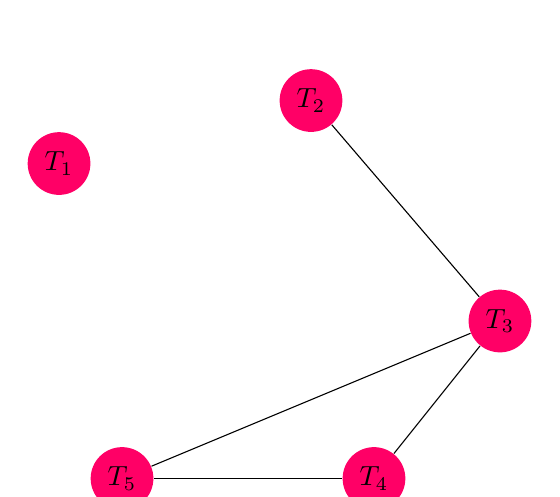
\begin{tikzpicture}[scale = 4]
	\node (a) at (0,1) [circle, fill = nicepink] {$T_1$};
	\node (b) at (0.8,1.2) [circle, fill = nicepink] {$T_2$};
	\node (c) at (1.4,0.5) [circle, fill = nicepink] {$T_3$};
	\node (d) at (1,0) [circle, fill = nicepink] {$T_4$};
	\node (e) at (0.2,0) [circle, fill = nicepink] {$T_5$};
	\draw (b) edge (c);
	\draw (c) edge (d);
	\draw (c) edge (e);
	\draw (d) edge (e);
	\end{tikzpicture}
	\end{center}
	\caption{A small network example}\label{toy_network}
\end{figure}
I think we can assume that
\[
p(\b{x}) = \prod_{s\sim t} \psi_{st}(\b{x})\prod_{s}\psi_s(\b{x})
\]
To start, we should think about the distribution of an independent node ($T_1$). Clearly
\[
P(T_1 = x) = \psi_{1}(x)
\]
Similarly, we should have
\[
P(T_2 = x) = \psi_2(x) = \int \psi_2(x)\psi_{23}(y) dy =  \bE (P(T_2 = x|T_3))   
\]
Maybe a binomial is a good idea:
\[
P\left(T_1 = \frac{k}{N}\right) = \binom{N}{k}p^k(1-p)^{N-k}
\]
where $p$ is something like the proportion of times $T_1$ appears in the data, the sum of abundances of $T_1$ in the data divided by $N$. $N$ is some scaling parameter, like the largest total abundance or something. But then, it's natural to take $N$ large and get a Gaussian by the CLT. So maybe we do a multivariate Guassian. Then
\[
\psi_{s\sim t}(\b{x}) = \exp\left(-\frac{1}{2} x_s \Lambda_{st}x_t\right)
\]
and
\[
\psi_s(\b{x}) = \exp\left(\eta_s x_s - \Lambda_{ss}x_s^2\right)
\]
\cite{machine_learning}. We already have the covariance (normalized by the product of the standard deviations) matrix $\Sigma$, in the Pearson coefficient. So, we have $\Lambda = \Sigma^{-1}$, and $\b{\eta} = \Sigma^{-1}\b{\mu}$. Unfortunately, $\Sigma$ is singular, it's dimension is bounded by the number of samples I have. This of course leaves us in the wind when it comes to $\Lambda$. So, I suppose we have to try to approximate $\Lambda$ subject to the constraint that if $s \not\sim t$, $\Lambda_{st} = 0$. We can use the SVD:
\[
\Sigma = M S N^* \Rightarrow \Sigma^+ = N \tilde{S} M^*
\] 
where $\tilde{S}$ is diagonal with $1/s_i$ until you get to zero singular values, where you just put a $0$. Because $\Sigma$ is symmetric, we have $M^* = N$. Then,
\[
\Sigma^+ = N \tilde{S} N
\]
I guess this is used, although it doesn't seem to preserve zeros. There's a function in scipy.

On the other hand, taking $N$ large and $p$ small we get an exponential random variable. So perhaps I want
\[
\psi_1(x) = e^{-\lambda}\frac{\lambda^{Nx}}{(Nx)!}
\]
or more directly
\[
\psi_1(x) = \binom{N}{Nx}p^{Nx}(1-p)^{N-Nx}
\]
and using Stirling's formula,
\[
\log(\psi_1) \approx N\left[x \log\left(\frac{p}{x}\right) + (1-x)\log\left(\frac{1-p}{1-x}\right)\right]
\]

\subsection{Comparing configurations without specifying $\psi$}
To compare two configurations $\b{x}$ and $\b{y}$, we can inspect
\[
\frac{P(\b{x})}{P(\b{y})} > 1
\]
without knowing them. For that, I would need to just identify which cliques change, and ask whether they increase or decrease. How exactly to decide that is a question. Probably single nodes we wouldn't change. For a clique, we could assume that $\psi_c$ decreases if we have over half the nodes and reduce and still have at least half, but increase if the we have less than half and decrease. That is, let $c$ be a clique with $n$ members, and $\psi_c(k)$ be the value of $\psi_c$ with $k$ members ``on". Then
\[
\frac{\psi_c(k+1)}{\psi_c(k)}   \left\{\begin{array}{c c}
>1 & k>\nicefrac{n}{2}\\
<1 & k\leq \nicefrac{n}{2}
\end{array}\right.
\]
Then, we are basically asserting the cliques like to either be all there or none there. Which seems good.

Here the algorithm for deciding which of two nodes should be on and which should be off would be:
\begin{enumerate}[(i)]
	\item Identify cliques $c_1,...,c_m$ which contain one or both nodes
	\item compute $\frac{\psi_{c_i}(k^1)}{\psi_{c_i}(k^2)}$ for each  $i \in \{1,...,m\}$, where $k^j$ is the number of members present in configuration $j \in \{1,2\}$, and this fraction is computed according to a simple rule of the kind above.
	\item multiply these ratios: $\frac{P(\text{configuration 1})}{P(\text{configuration 2})} = \prod_{i=1}^k \frac{\psi_{c_i}(k^1)}{\psi_{c_i}(k^2)}$
\end{enumerate}

I need to specify that rule. The simplest reasonable thing is probably linear
\[
\frac{\psi_c(k+1)}{\psi_c(k)} = \frac{2(1-r_{min})}{n - 1} k + r_{min}
\]
but one could imagine some kind of sigmoidal rule as well, so that around $\nicefrac{n}{2}$ this ratio is close to $1$. This makes sense on a $2$ clique, as it implies that
\[
\psi(2) > \psi(1) \; \& \; \psi(0) > \psi(1)
\]
and in general makes sense for $n$ even. It makes sense for $n$ odd as well. It asserts that it is equally likely to have on $\nicefrac{n}{2} \pm \nicefrac{1}{2}$. Finally, if we need to compare $k$ and $k+2$, we simply take
\[
\frac{\psi(k+2)}{\psi(k)} = \frac{\psi(k+2)}{\psi(k+1)}\frac{\psi(k+1)}{\psi(k)}
\]
That is, a discrete analogue to the chain rule.

To compare $P(v_1 =1 | \xi)$ and $P(v_2 = 1 | \xi)$, let $X$ be the configurations with $\xi$ and $v_1 = 1$, and $Y$ the configurations with $\xi$ and $v_2 = 1$. Then,
\[
P(v_1 = 1| \xi) = \sum_{x\in X} \frac{P(x)}{P(\xi)}
\]
and so
\[
P(v_1 = 1| \xi) > P(v_2 = 1|\xi) \Leftrightarrow \sum_{x\in X\setminus Y} P(x) >\sum_{y \in Y\setminus X} P(y)
\]
but inspecting $X$ and $Y$, we see that this is equivalent to 
\[
\sum_{x\in X\setminus Y} (P(x) - P(\tilde{x})) > 0
\]
where $\tilde{x} = x$ for all nodes except $v_1$ and $v_2$, while $x(v_1) = \tilde{x}(v_2) = 1$ and $x(v_2) = \tilde{x}(v_1) = 0$. This can be written
\begin{equation}
\sum_{x\in X\setminus Y}\prod_{c:v_1,v_2 \not \in c}\psi_c(x)\left(\prod_{c:v_1\text{ or }v_2  \in c}\psi(x) - \prod_{c:v_1\text{ or }v_2  \in c}\psi(\tilde{x}) \right) >0
\end{equation}
where $c$ are maximal cliques of the RMF.


\subsection{Diffusion based method.}
Here's an idea inspired by spectral clustering: Solve the diffusion equation on the graph:
\[
\frac{\partial}{\partial t} u(v,t) = L u(v,t)
\]
where $v$ takes values in the vertex set of the graph. Then, we can encode ``known" information in three ways: initial values, boundary values, or a forcing vector.

\begin{inbox2}
\begin{method}[Initial Value Problem]\label{initalCond}
Let $u_i(t)$ be the solution at node $v_i$ to the discete diffusion problem
\[
\frac{d}{dt}\b{u}(t)  = - L\b{u}
\]
where $L$ is the  graph laplacian with initial conditions $u_i = 1$ if node $v_i$ is known to be ``on", $u_j = 0$ if $v_j$ is known to be ``off", and $u_k = 0.5$ (or $0$, or perhaps encoded with some confidence in $[0,1)$) if $v_k$ is unknown. We then normalize the initial vector so that it represents a probability distribution on the nodes.

Then, if $\b{K}$ is the information ``known" and the values of $v_{k}$ and $v_{l}$ are unknown,
\[
\int_0^{\infty} u_k(t) dt - \int_0^{\infty} u_l(t) dt >  0 \Rightarrow  P(v_k=  1|\b{K}) > P(v_l = 1|\b{K})
\]
\end{method}
\end{inbox2}
We can easily compute these comparisons. Solutions to the diffusion equation are of the form
\[
\b{u} = \sum_{i=1}^a c_i \b{1} + \sum_{i=a+1}^n c_i e^{\lambda_i t} \b{\xi}_i 
\]
where $a$ is the number of connected components of the graph, and $\lambda_i,\b{\xi}_i$ are eigenvalue, eigenvector pairs of $L$. Note that each eigenvalue $\lambda_i \leq 0$, with $\lambda_i<0$ for $i = a+1,...,n$ \cite{vonLuxburg2007}. Then, assuming there is some intial mass on the connected components containing $v_1$ and $v_2$, 
\[
\int_0^{\infty} u_k(t) dt - \int_0^{\infty} u_l(t) dt =   \sum_{i=a+1}^n c_i  (v_{ik} - v_{il}) \int_0^{\infty} e^{\lambda_i t} dt = \sum_{i=a+1}^n \frac{-c_i}{\lambda_i}  (\xi_{il} - \xi_{ik}) 
\]
and $\b{c} = V^{-1}\b{u}(0)$. Therefore, it is straightforward to compute and compare the transitive terms of the solution:
\[
\int_0^{\infty}\left( u_k(t) - \sum_{i=1}^a c_i \right) dt = \sum_{i=a+1}^n \frac{-c_i}{\lambda_i}\xi_{ik}
\]


We can regard this method as the Kolmogorov forward equation of a jump process that transitions from taxa to taxa which have an edge between them at a linear rate (see \cref{kfor}). The state space of this process is the affine space $\b{1}^{\perp} + \b{b}_1\cap \bZ^n_{\geq 0}$, where $\b{b}_i$ are the standard basis vectors. At any time $t$, $u_l(t)$ is the probability that the process is in the state $\b{e}_l$. This model clearly admits no extinction events and is complex balanced deficiency zero. In the deterministic setting, it has globally attracting equilibrium $\frac{1}{n}\b{1}$. Therefore, according to \cite{Anderson2010}, it has stationary distribution on each connected component
\[
\pi(\b{x}) = \frac{1}{Z_{cc}} \prod_{i=1}^n \frac{\left(\frac{1}{n}\right)^{x_i}}{x_i!}e^{-\frac{1}{n}}
\]
The state space of the system is $\{\b{b}_j\}$, and we note that for $j = 1,...,a$
\[
c_j = \pi(\b{b}_j) = \frac{1}{Z_{cc} n}e^{-\frac{1}{n}}
\]
and so the distribution is uniform on each conected component. If it is higher on one connected  component than an other, the above integral will be larger on that component. To compare within a connected component of the graph, we must look at the transient behavior, which we take by the integral above, subtracting this stationary distribution. This is going to allow us to compare nodes in the same connected component. We are choosing first the most likely connected components and then ranking within those by transient behavior. 

Interestingly, we can regard this as the reaction network directly, deterministically modeled, which is the volume scaling limit of the jump process described above.

This method is the only one of the three that is well suited for judging the entire network, without confidence in the preknowledge encoded in the initial conditions. The other two require at least one (\cref{boundarVal}) or two (\cref{forcing}) confident assertion for each connected component of the graph.

\begin{inbox2}
	\begin{method}[Boundary Value Problem]\label{boundarVal}
Let $u_i(t)$ be the solution at node $v_i$ to the discete diffusion problem
\[
\frac{d}{dt}\b{u}(t)  = - L\b{u}
\]
where $L$ is the  graph laplacian with fixed values (which can be regarded as boundary values) $u_i = 1$ if node $v_i$ is known to be ``on", $u_j = 0$ if $v_j$ is known to be ``off". 

Then, if $\b{K}$ is the information ``known" and the values of $v_{k}$ and $v_{l}$ are unknown, and $\b{\tilde{u}}$ is the equilibrium solution to the diffusion problem,
\[
\tilde{u}_k dt >  \tilde{u}_l \Leftrightarrow  P(v_k=  1|\b{K}) > P(v_l = 1|\b{K})
\]
	\end{method}
\end{inbox2}

First, we establish conditions under which the boundary value version will always have an equilibrium. A ``boundary value" set on the graph is a set of fixed node values. We have seen already that the equilibrium of the diffusion problem is uniform, and so if we only have known ``on" nodes $\b{\tilde{u}} = \b{1}$.  If we specify off nodes as well, then there is not an equilibrium solution to the diffusion problem which gives those values at boundary nodes. However, this doesn't mean the boundary value problem (or, more precisely, the equvalent forced problem on the unknown subset) doesn't have an equilibrium solution. Take for example a complete graph on three nodes. If we prescribe one node as $1$ and one as $0$, the reduced problem is
\[
\frac{d}{dt} u = -2u + 1
\]
which has an equilibrium at $u = \nhalf$. This is not an equilirium to the entire problem, because in that case
\[
-L\begin{pmatrix}
1 \\ \nhalf \\ 0
\end{pmatrix} = \begin{pmatrix}
-2 & 1 & 1\\ 1 & -2 & 1 \\ 1 & 1 & -2
\end{pmatrix}\begin{pmatrix}
1 \\ \nhalf \\ 0
\end{pmatrix} = \begin{pmatrix}
-\nicefrac{3}{2} \\ 0 \\ \nicefrac{3}{2}
\end{pmatrix}
\]
The boundary value problem is equivalent to the forced problem on unknown nodes
\[
\frac{d}{dt}\b{u}|_{\b{U}} = L|_{\b{U}}\b{u} + f_{\b{K}}
\]
where $\b{u}|_{\b{U}}$ is the projection of $\b{u}$ onto the unknown set of nodes, $L|_{\b{U}}$ is $L$ with the rows and columns of the known nodes removed, and $f_{\b{K}}$ is the forcing due to the boundary conditions.
	
The nullity of $L$ is the number of connected components of the graph. Removing a column from a matrix will not lower the rank of that matrix if the column was a linear combination of other columns, which is the case precisely when the column is the first one removed that corresponds to some connected component of the graph. Therefore, as long as we specify at least one ``boundary value" from each connected component, $L|_{\b{U}}$ is non-singular and there exists a unique equilibrium to the boundary value problem.

The equilibrium is simply computed by solving 
\[
0 = L|_{\b{U}}\b{\tilde{u}} + f_{\b{K}}
\]

The boundary value problem can be interpreted as a population walking around the graph, with the population at some nodes maintained at fixed values. We then assume that probability that a node is ``on" is proportional to the size of the population at that node. Perhaps ``voters" are a good analogy. 

It can also be interpreted as the same reaction network as \cref{initalCond}, but the values of some species fixed.

\begin{inbox2}
\begin{method}[Forced Problem]\label{forcing}
Let $u_i(t)$ be the solution at node $v_i$ to the discete diffusion problem
\[
\frac{d}{dt}\b{u}(t)  = - L\b{u} + f
\]
where $L$ is the  graph laplacian and $f$ a forcing vector with $f_i = \alpha_{cc}$ if node $v_i$ is known to be ``on", $f_j = -\beta_{cc}$ if $v_j$ is known to be ``off", where $cc$ denotes a connected component of the graph. We choose $\alpha_{cc}$ and $\beta_{cc}$ so that on any connected component $cc$, $\sum \alpha_{cc}= \sum \beta_{cc}= 1$. 

Then, if $\b{K}$ is the information ``known" and the values of $v_{k}$ and $v_{l}$ are unknown, and $\b{\tilde{u}}$ is the equilibrium solution to the diffusion problem,
\[
\tilde{u}_k dt >  \tilde{u}_l \Leftrightarrow  P(v_k=  1|\b{K}) > P(v_l = 1|\b{K})
\]
\end{method}
\end{inbox2}

Notice that the kernel of $L$ is $\mathit{span}(\{\b{1}|_{cc}\})$, where $cc$ denotes a connected component of the graph. For an equilibrium solution to exist, any connected component with an ``on" node must also have an ``off" node, so that $f \in \mathit{span}(\{\b{1}|_{cc}\})^{\perp}$, which is the range of $L$ because $L$ is symmetric. 

We can easily compute the equilibrium solution by solving, as long as we have guarenteed that $f \in \mathit{range}(L)$. On a practical note, we use numpy's least squares solver because the matrix $L$ is singular. Unfortunately, if we do not specify an off node in a connected component in which we do specify an on node (or vice versa), there is no equilibrium solution.

The third method can be interpreted much like \cref{boundarVal}. However, instead of the population being maintained at known nodes, we have a constant inflow or outflow from the graph at these nodes. 

This can also be regarded as the same chemical reaction network model as \cref{initalCond}, but now with inflow and outflow. 

\begin{figure}
	\begin{subfigure}[b]{0.5\linewidth}
			\begin{center}
			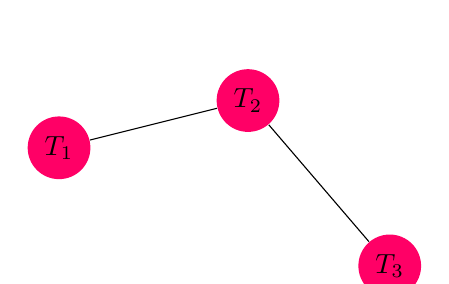
\begin{tikzpicture}[scale = 3]
			\node (a) at (0,1) [circle, fill = nicepink] {$T_1$};
			\node (b) at (0.8,1.2) [circle, fill = nicepink] {$T_2$};
			\node (c) at (1.4,0.5) [circle, fill = nicepink] {$T_3$};
			\draw (b) edge (c);
			\draw (a) edge (b);
			\end{tikzpicture}
		\end{center}
		\caption{A small network example}
	\end{subfigure}
	\begin{subfigure}[b]{0.5\linewidth}
		\begin{center}
			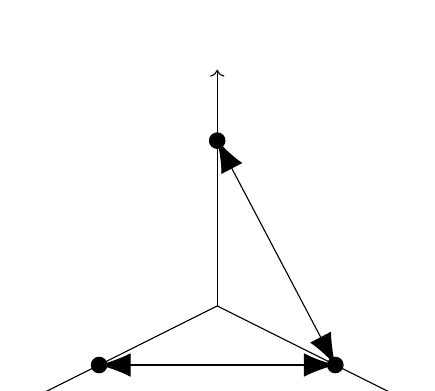
\begin{tikzpicture}[scale = 3]
				\draw[->] (0,0)--(0,1);
				\draw[->] (0,0)--(0.8,-0.4);
				\draw[->] (0,0)--(-0.8,-0.4);
				\fill (0,0.7) circle (1 pt);
				\fill (0.5,-0.25) circle (1 pt);
				\fill (-0.5,-0.25) circle (1 pt);
				\draw[{Latex[length=4mm]}-{Latex[length=4mm]}] (0,0.7) -- (0.5,-0.25);
				\draw[{Latex[length=4mm]}-{Latex[length=4mm]}] (0.5,-0.25) -- (-0.5,-0.25);
				\end{tikzpicture}
		\end{center}
	\caption{State transition graph for the IVP}
\end{subfigure}
\caption{Diffusion is equivalent to the Kolmogorov forward equations for the above system.}\label{kfor}
\end{figure}



\subsubsection{Tests of these methods}
I tested these three ideas on two small (unweighted) graphs, shown in \cref{tests}.

\begin{figure}
		\begin{subfigure}[b]{0.33\linewidth}
		\begin{center}
			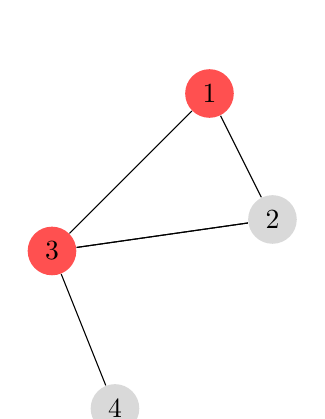
\begin{tikzpicture}[scale = 2]
			\node (a) at (1,2) [circle, fill = nicered] {$1$};
			\node (b) at (1.4,1.2) [circle, fill = lgray] {$2$};
			\node (c) at (0,1) [circle, fill = nicered] {$3$};
			\node (d) at (0.4,0) [circle, fill = lgray] {$4$};
			\draw (b) edge (c);
			\draw (a) edge (b);
			\draw (a) edge (c);
			\draw (b) edge (c);
			\draw (c) edge (d);
			\end{tikzpicture}
		\end{center}
		\caption{One tested configuration}
	\end{subfigure}
		\begin{subfigure}[b]{0.33\linewidth}
	\begin{center}
		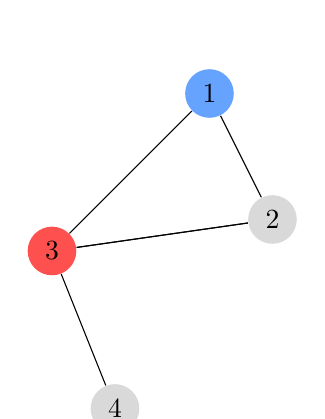
\begin{tikzpicture}[scale = 2]
		\node (a) at (1,2) [circle, fill = lblue] {$1$};
		\node (b) at (1.4,1.2) [circle, fill = lgray] {$2$};
		\node (c) at (0,1) [circle, fill = nicered] {$3$};
		\node (d) at (0.4,0) [circle, fill = lgray] {$4$};
		\draw (b) edge (c);
		\draw (a) edge (b);
		\draw (a) edge (c);
		\draw (b) edge (c);
		\draw (c) edge (d);
		\end{tikzpicture}
	\end{center}
	\caption{One tested configuration}
\end{subfigure}
	\begin{subfigure}[b]{0.33\linewidth}
		\begin{center}
			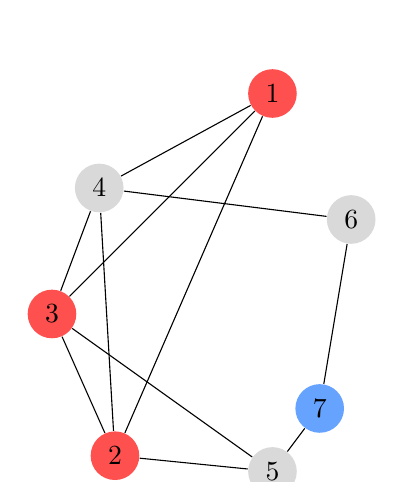
\begin{tikzpicture}[scale = 2]
			\node (a) at (1,2.3) [circle, fill = nicered] {$1$};
			\node (b) at (0,0) [circle, fill = nicered] {$2$};
			\node (c) at (-0.4,0.9) [circle, fill = nicered] {$3$};
			\node (d) at (-0.1,1.7) [circle, fill = lgray] {$4$};
			\node (e) at (1,-0.1) [circle, fill = lgray] {$5$};
			\node (f) at (1.5,1.5) [circle, fill = lgray] {$6$};
			\node (g) at (1.3,0.3)[circle, fill = lblue] {$7$};
			\draw (a) edge (b);
			\draw (a) edge (c);
			\draw (a) edge (d);
			\draw (b) edge (c);
			\draw (b) edge (d);
			\draw (c) edge (d);
			\draw (d) edge (f);
			\draw (f) edge (g);
			\draw (e) edge (g);
			\draw (c) edge (e);
			\draw (b) edge (e);
			\end{tikzpicture}
		\end{center}
		\caption{One tested configuration}
	\end{subfigure}
	\caption{Test networks. Gray nodes were ``unknown", blue nodes ``off", and red ``on".}\label{tests}
\end{figure}

\begin{table}
	\begin{center}
\begin{tabular}{|l|l|l|l|}
	\hline Configuration & Method & Ranking & Ties\\
	\hline
	\cref{tests}(a) &  IVP & 2, 4 & none  \\ \cline{2-4}
	 & BVP & 4, 2 & 4, 2 \\ \cline{2-4}
	 & Forcing & 2, 4 & none \\
	\hline
		\cref{tests}(b) &  IVP & 4, 2 &none \\ \cline{2-4}
	& BVP &4, 2 & none  \\ \cline{2-4}
	& Forcing &4, 2 & none\\
	\hline
		\cref{tests}(c) &  IVP & 4, 5, 6& none \\ \cline{2-4}
	& BVP & 4, 5, 6&  none\\ \cline{2-4}
	& Forcing &  4, 5, 6& none \\
	\hline
\end{tabular}
\end{center}
\caption{Results of ranking nodes by liklihood of being ``on" by the three above methods}\label{rankres}
\end{table}
	
I also tested these methods on a genus level network built from Pearson correlation higher than $0.8$ with $p < 0.05$ (determined by Monte Carlo simulation). This network had a number of connected components. I used a column of the sample data used to creat the network as my configuration, with nodes with larger than mean abundance take ``on" and no abundance taken ``off", while taxa with non-zero but below mean abundance taken as ``unknown". By analysing all nodes using \cref{initalCond} (\cref{diffusion_sample} (a)), positive likelihood can be assigned to nodes assumed ``off" if they are connected to nodes assumed ``on". In the other two methods, only unkown and nodes assumed on can have positive likelihood (\cref{diffusion_sample} (b)).

\begin{figure}
	\begin{center}
	\begin{subfigure}[b]{0.48\linewidth}
	\begin{center}
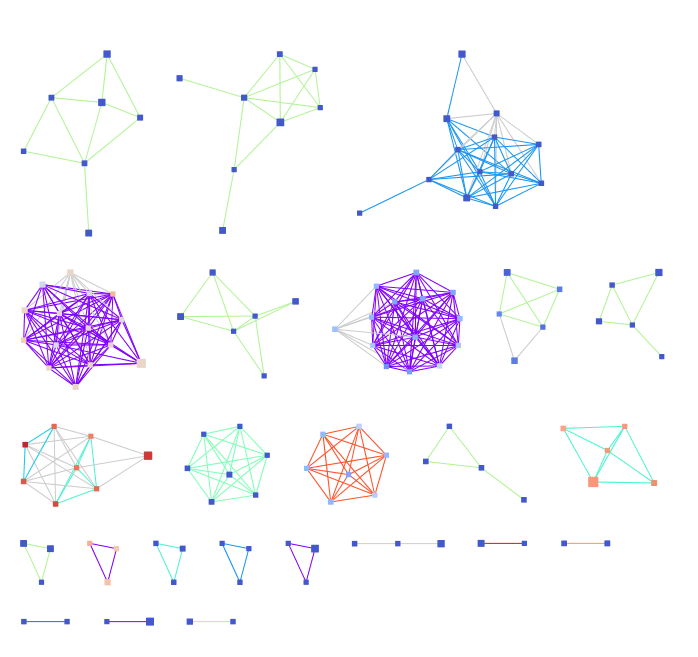
\includegraphics[scale = 0.3]{ranked_ivp.png}	
\end{center}
\caption{Result of \cref{initalCond}, with all nodes analyzed. Hotter colors indicate higher likelihood.}
\end{subfigure}
\begin{subfigure}[b]{0.48\linewidth}
		\begin{center}
		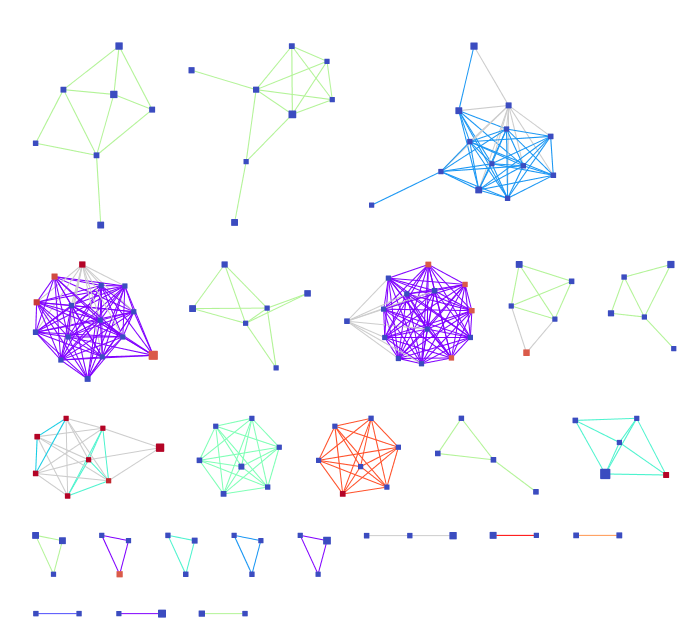
\includegraphics[scale = 0.3]{ranked_bdvp.png}	
	\end{center}
	\caption{Result of \cref{boundarVal}. Hotter colors indicate higher likelihood, with red indicating assumed ``on".}
\end{subfigure}
\begin{subfigure}[b]{0.48\linewidth}
		\begin{center}
		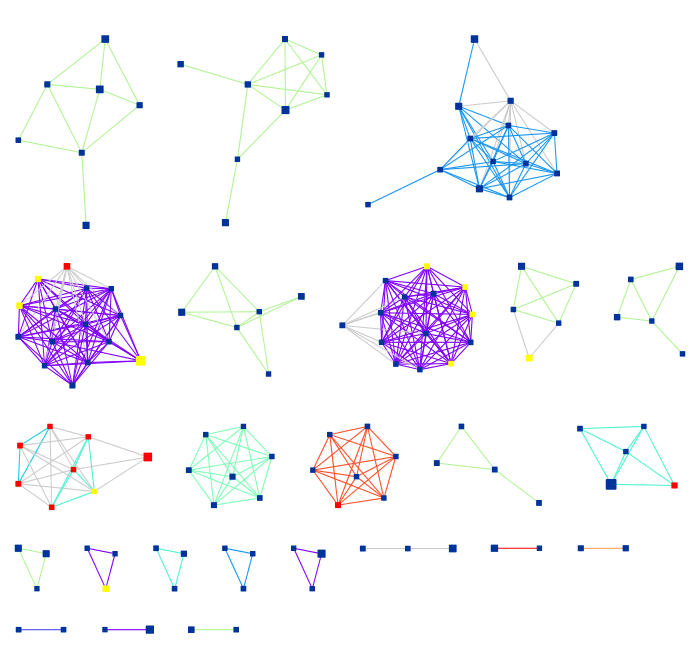
\includegraphics[scale = 0.3]{ranked_known_nodes.png}	
	\end{center}
	\caption{The ``known" set - blue is off and red is on, while yellow is unknown.}
\end{subfigure}
\caption{Result of diffusion methods. Edge color represents the shared sample type of the nodes (i.e. samply type the taxa was found most often in), with gray indicating different types.}\label{diffusion_sample}
\end{center}
\end{figure}	

\subsection{Read based analysis}
Another way to think about the question of which taxa are present given a sample is to think specifically about the reads, and which taxa produce them. This would give us a ``reaction network" of the type 
\[
\xymatrix@R = 1 pt{
t_1 \ar[r] \ar[ddr] & r_1	\\
t_2 \ar[r] \ar[ur] & r_2\\
t_3 \ar[r] \ar[dr] \ar[uur] & r_3\\
 & r_4}
\]
Then, what we observe is the equilibrium condition of the reaction network, and we want to determine the initial condition. Or, perhaps we treat it as an I/O system in which we observe the output and want to know the input.


	
\section{Comparison of Networks}
At some point here, I'm going to want to compare networks. Luckily, there's things to do. There are of course the simple and obvious: size, radius, various connectivity and clustering metrics. There are also more interesting things, like the random walk kernel on graphs. Graph kernels are similar to an inner product on two graphs.

A graph kernel $k(G_1,G_2)$ must be symmetric and positive definite (an inner product must also be bilinear) \cite{Vishwanathan}. To compute the most common type (random walk kernels) we need to define the direct product of two graphs $G$ and $G'$. That is the graph $G_{\times}$ with vertices 
\[
(v_i,v_j') \in V \times V'
\]
and edges
\[
(v_i,v_j') \sim (v_k,v_l') \Leftrightarrow v_i \sim v_k \, \&\, v_j' \sim v_l'
\]
We can compute the adjacency matrix of this by computing the Kronecker product of the adjacency matrices of $G$ and $G'$. The Kronecker product of matrices $A$ and $B$ is
\[
A \otimes B = \begin{pmatrix}
a_{11} B & a_{12}B & \cdots & a_{1m}B\\
a_{21}B & \ddots & &\\
\vdots & & & \\
a_{n1}B & & & a_{nm}B
\end{pmatrix}
\]
A random walk on this graph is isomorphic to a random walk on either graph, and so one can consider a random walk on this graph as a simultaneous random walk on both. We can take the adjacency matrices normalized so row sums are 1, call those $A$, $A'$, and then
\[
W_{\times}  = A \otimes A'
\] 
This gives a stochastic matrix $W_{\times}$. Given distributions $p$ and $p'$, define $p_{\times}  = p \otimes p'$. Define the kernel
\[
k(G,G') = \sum_{k=0}^{\infty} \mu(k) q_{\times}^T W_{\times}^k p_{\times}
\]
where $q,q'$ are stopping probabilities, and $p,p'$ are initial distributions. This counts all the common random walks. The coefficients $\mu(k)$ serve two purposes. One is to make sure the sum is finite. The other allows one to tune the kernel to emphasize walks of certain lengths. I think it's called geometric if $\mu(k) = c^k$. However, this seems like it will overemphasize short walks, of which there will be many in common.

	
\bibliographystyle{plain}
\bibliography{../../summer17}
\end{document}